\chapter{COATI: STATISTICAL PAIRWISE ALIGNMENT OF PROTEIN CODING SEQUENCES}
\label{ch:alignpair}

% \section{Abstract}
% Sequence alignment is an essential method in bioinformatics and the basis of many analyses, including phylogenetic inference, ancestral sequence reconstruction, and gene annotation.
% Sequence artifacts and errors made in alignment reconstruction can impact downstream analyses leading to erroneous conclusions in comparative and functional genomic studies.
% For example, abiological frameshifts and early stop codons are common artifacts found in protein coding sequences that have been annotated in reference genomes.
% While such errors are eventually fixed in the reference genomes of model organisms, many genomes used by researchers contain these artifacts, and researchers often discard large amounts of data in comparative genomic studies to prevent artifacts from impacting results.
% To address this need, we present COATi, a statistical, codon-aware pairwise aligner that supports complex insertion-deletion models and can handle artifacts present in genomic data.
% COATi allows users to reduce the amount of discarded data while generating more accurate sequence alignments.

\section{Introduction}

Sequence alignment is a fundamental task in bioinformatics and a cornerstone step in comparative and functional genomic analysis \citep{sequence_alignment_rosenberg_2009}. While sophisticated advancements have been made, the challenge of alignment inference has not been fully solved \citep{art_morrison_2015}.
%
The alignment of protein-coding DNA sequences is one such challenge, and a common approach to this problem is to perform alignment inference in amino-acid space (e.g.\ \citealt{bininda2005transalign,abascal2010translatorx}).
While this approach is an improvement over DNA models, it discards information, underperforms compared to alignment at the codon level, and fails in the presence of artifacts such as frameshifts and early stop codons.
Although some aligners incorporate codon substitution models, they do not support frameshifts or lack a statistical model.
In addition, existing aligners typically force gaps to occur between codons, whereas in natural sequences, only about 42\% of indels occur between codons \citep{taylor2004occurrence,zhu2022profiling}.
This mismatch between aligner assumptions and biology can produce sub-optimal alignments and inflated estimates of sequence divergence (Fig.\ \ref{fig:aln}).

% Figures are 86 mm or 178 mm wide
\begin{figure}[!ht]
    \centering%
    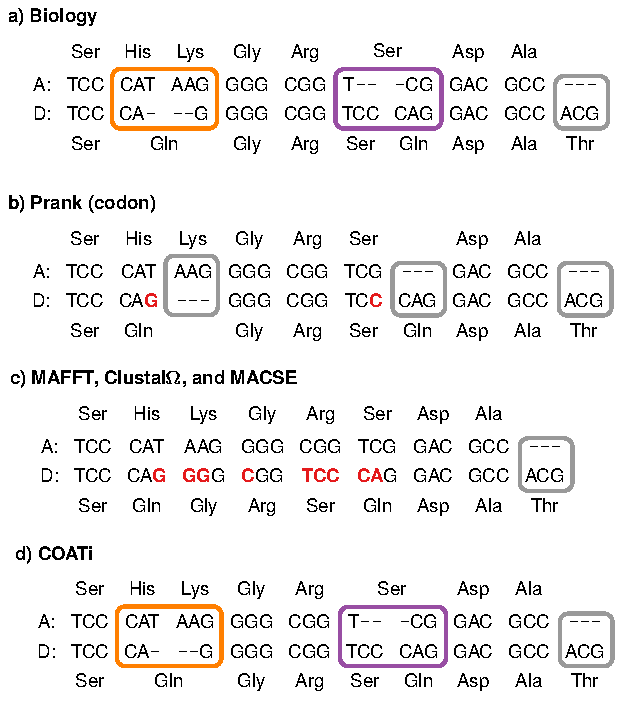
\includegraphics[scale=1]{fig-aln.pdf}
    \par
    \caption[Suboptimal alignments and indel phases]{
        Standard algorithms produce suboptimal alignments.
        (a) shows the true alignment of an ancestor sequence (A) and a descendant sequence (D).
        (b), (c), and (d) are the results of different aligners.
        Nucleotide mismatches are highlighted in red. Phase 0, phase 1, and phase 2 indels are shown in gray, purple, and orange, respectively.
        Additionally, the orange indel is type II (an amino-acid indel plus an amino-acid change) while the purple indel is type I (an amino-acid indel only).
        COATi is the only aligner able to retrieve the biological alignment in this example.
        }
    \label{fig:aln}
\end{figure}

Genome quality impacts conclusions drawn from comparative genomic studies, and uncorrected errors in the alignment stage can lead to erroneous results in comparative and functional genomic studies \citep{estimates_schneider_2009,effect_fletcher_2010,hubisz2011error}.
Genomes for model organisms often get refined over many iterations and achieve high quality with meticulously curated protein coding sequences.
In contrast, genomes for non-model organisms might only receive partial curation and typically have lower-quality sequences and annotations.
These genomes often lack the amount of sequencing data needed to fix artifacts, including missing exons, erroneous mutations, and indels \citep{jackman2018tigmint}.
%
When comparative and functional genomics studies include data from non-model organisms, care must be taken to identify and manage such artifacts; however,
current alignment methods are ill-equipped to handle common artifacts in genomic data, requiring costly curation practices that discard significant amounts of information.
To address this problem, I developed COATi, short for COdon-aware Alignment Transducer, a pairwise statistical aligner that incorporates codon substitution models and is robust to artifacts present in modern genomic data.

\section{Materials}

\subsection{Finite State Transducers}

Statistical alignment is typically performed using pairwise hidden Markov models (pair-HMMs), which have the ability to rigorously model molecular sequence evolution \citep{bradley2007transducers}.
Pair-HMMs are computational machines with probabilities for emitting symbols from the states to two output tapes and probabilities for the transitions between the states (arcs). Each tape represents a sequence and a path through these computational machines is a possible pairwise alignment. Pair-HMMs contain a finite number of states, typically labeled match (M), insert (I), and delete (D). The emission probability distribution of M usually follows a substitution model for emitting an aligned pair or symbols ($s_i,v_j$) from sequences $s$ and $v$. States I and D have distributions for emitting symbols against a gap (-). In addition, arcs in pair-HMMs have transition probabilities. Figure \ref{fig:hmm} illustrates a common pair-HMM architecture, with affine gap scoring. Conceptually, these machines generate two sequences, $s$ and $v$, from an unknown ancestor and can calculate the probability that two sequences are related, represented by $P(s, v)$ \citep{yoon_2009_hmm}.

\clearpage

\begin{figure}[!ht]
    \centering
    \resizebox{0.8\textwidth}{!}{% % !TEX program=lualatex
\definecolor{colorR}{RGB}{228,26,28}    % RED
\definecolor{colorB}{RGB}{55,126,184}   % BLUE
\definecolor{colorG}{RGB}{77,175,74}    % GREEN
\definecolor{colorP}{RGB}{152,78,163}   % PURPLE
\definecolor{colorO}{RGB}{255,127,0}    % ORANGE
\definecolor{colorY}{RGB}{255,255,51}   % YELLOW
\definecolor{colorBn}{RGB}{166,86,40}   % BROWN
\definecolor{colorPk}{RGB}{247,129,191} % PINK
\definecolor{colorGy}{RGB}{153,153,153} % GRAY

\tikzstyle{line}=[draw, -stealth', very thick]
\tikzstyle{block}=[circle,fill=colorB!50,on grid,font=\large]
\tikzstyle{lab}=[]
\tikzstyle{w}=[lab,midway]
\tikzstyle{e}=[lab,midway,auto=false,fill=colorP!50,font=\scriptsize]

\begin{tikzpicture}[node distance=40mm, auto,
	dottedline/.style = {ultra thick, loosely dotted,shorten >=1mm, shorten <=1mm}]
%%% Legend

%%% Indel FST
\node[block,align=center] (M) {\textbf{M}\\$s_i,v_j$};
\node[block,above right=25mm and 25mm of M,align=center] (I) {\textbf{I}\\$-,v_j$};
\node[block,below right=25mm and 25mm of M,align=center] (D) {\textbf{D}\\$s_i,-$};

\draw[line] (M) to[out=90,in=180] node[w,left=5mm] {$\delta$} (I);
\draw[line] (I) to[out=270,in=10] node[w,right=2mm] {$1-\varepsilon$} (M);

\draw[line] (M) to[out=270,in=180] node[w,left=5mm] {$\delta$} (D);
\draw[line] (D) to[out=90,in=350] node[w,right=2mm] {$1-\varepsilon$} (M);

\draw[line] (M.135) arc (45:302:8mm) node[w,left] {$1-2\delta$};
\draw[line] (I.45) arc (135:-120:8mm) node[w,right] {$\varepsilon$};
\draw[line] (D.45) arc (135:-122:8mm) node[w,right] {$\varepsilon$};

\node[font=\footnotesize,text width=50mm,below=4cm of M] (sequences) {
\begin{tabular}{r@{\,: }l}
\multicolumn{2}{l}{\textbf{Sequences}}\\
    \hline
	% X & input nucleotides\\
	% Y & intermediate nucleotides\\
	$s,v$ & sequences\\
	% \O & nothing/empty sequence\\
\end{tabular}
};

\node[font=\footnotesize,right=0.5cm of sequences,text width=50mm] {
\begin{tabular}{r@{\,: }l}
\multicolumn{2}{l}{\textbf{Parameters}}\\
\hline
	$\delta$ & gap open weight\\
	$\varepsilon$ & gap extension weight\\
\end{tabular}
};


\end{tikzpicture}

}
    \caption[Pair-HMM]{Example of a typical pair hidden Markov model (pair-HMM) used in statistical pairwise sequence alignment. Sequences $s$ and $v$ are aligned using an affine gap scoring model and a substitution model (unspecified). The arcs are weighted with gap opening parameter $\delta$ and gap extension $\varepsilon$, therefore defining no gap opening weight as $1-\delta$ and gap closing as $1-\varepsilon$.}
    \label{fig:hmm}
\end{figure}

A limitation of pair-HMMs is that they only model the evolution of two related sequences from an unknown ancestor.
Finite-state transducers (FSTs) have similar benefits to pair-HMMs with the additional feature that they can model the generation of a descendant sequence given an ancestral one.
FSTs, similar to pair-HMMS, are computational machines with a symbol alphabet, a set of states, and weighted arcs defining the transition probabilities between states. However, FSTs consume symbols from an input and emit symbols to an output tape ($a:b$), as opposed to having two output tapes ($a,b$). Properly weighted, an FST can calculate the probability that a descendant sequence, $v$, evolved from an ancestral sequence, $s$, represented by $P(v | s)$.

Furthermore, well-established algorithms for combining FSTs in different ways, including concatenation, composition, intersection, union, or reversal, allow the design of complex models by combining simpler FSTs \citep{bradley2007transducers,silvestre2021machine}.
Specifically, composition is a powerful and versatile algorithm for comparative sequence analysis, consisting of sending the output of one FST into the input of a second FST.
Composition allows combining two or more FSTs to create a new, more complex transducer. Figure \ref{fig:transcription} illustrates how DNA transcription for a codon can be achieved by composing a complimenting FST with a transducer that replaces thymines with uracil, where the three nucleotides are read and complimented in \ref{fig:transcription}-a, which are then used as the input of \ref{fig:transcription}-b, resulting in the transcription of the codon (Fig.~\ref{fig:transcription}-c). COATi uses composition to derive a statistical alignment model from the combination of smaller FSTs, each representing a specific process.

\begin{figure}[!ht]
    \centering
    \hspace*{-3.5em}\resizebox{1.05\textwidth}{!}{\definecolor{colorR}{RGB}{228,26,28}    % RED
\definecolor{colorB}{RGB}{55,126,184}   % BLUE
\definecolor{colorG}{RGB}{77,175,74}    % GREEN
\definecolor{colorP}{RGB}{152,78,163}   % PURPLE
\definecolor{colorO}{RGB}{255,127,0}    % ORANGE
\definecolor{colorY}{RGB}{255,255,51}   % YELLOW
\definecolor{colorBn}{RGB}{166,86,40}   % BROWN
\definecolor{colorPk}{RGB}{247,129,191} % PINK
\definecolor{colorGy}{RGB}{153,153,153} % GRAY

\tikzstyle{line}=[draw, -stealth', very thick]
\tikzstyle{block}=[circle,fill=colorB!50,on grid]
\tikzstyle{lab}=[]
\tikzstyle{w}=[lab,midway]
\tikzstyle{e}=[lab,midway,below=-4mm,auto=false,font=\scriptsize]

% \begin{document}
% \begin{tikzpicture}[node distance=25mm, auto]
\begin{tikzpicture}[node distance=25mm, auto,
	dottedline/.style = {ultra thick, loosely dotted,shorten >=1mm, shorten <=1mm}]

% complimenting FST
\node (titlea) {\textbf{a) DNA Complement}};

\node[block,below left=1.5cm and -10mm of titlea.west,fill=colorG!50] (start1) {start};
\node[block,right=15mm of start1,minimum size=20pt] (cod0) {};
\node[block,right=20mm of cod0,minimum size=20pt] (cod1) {};
\node[block,right=20mm of cod1,minimum size=20pt] (cod2) {};
\node[block,right=20mm of cod2,minimum size=20pt] (cod3) {};
\node[block,fill=colorR!50,right=15mm of cod3] (end1) {end};

\draw[line] (start1) -- (cod0);
\draw[line] (cod3) -- (end1);

\draw[line] (cod0) to[bend right=-60] node[e] {A:T} (cod1);
\draw[line] (cod0) to[bend right=-25] node[e] {C:G} (cod1);
\draw[line] (cod0) to[bend right=25] node[e,below=-4.5mm] {G:C} (cod1);
\draw[line] (cod0) to[bend right=60] node[e] {T:A} (cod1);

\draw[line] (cod1) to[bend right=-60] node[e] {A:T} (cod2);
\draw[line] (cod1) to[bend right=-25] node[e] {C:G} (cod2);
\draw[line] (cod1) to[bend right=25] node[e,below=-4.5mm] {G:C} (cod2);
\draw[line] (cod1) to[bend right=60] node[e] {T:A} (cod2);

\draw[line] (cod2) to[bend right=-60] node[e] {A:T} (cod3);
\draw[line] (cod2) to[bend right=-25] node[e] {C:G} (cod3);
\draw[line] (cod2) to[bend right=25] node[e,below=-4.5mm] {G:C} (cod3);
\draw[line] (cod2) to[bend right=60] node[e] {T:A} (cod3);

% T->U
\node[right=6cm of titlea] (titleb) {\textbf{b) Replacing thymine with uracil}};

\node[block,below right=1.5cm and 12mm of titleb.west,fill=colorG!50] (start2) {start};
\node[block,right=20mm of start2,minimum size=30pt] (cod4) {};
\node[block,fill=colorR!50,right=20mm of cod4] (end2) {end};

\draw[line] (start2) -- (cod4);
\draw[line] (cod4) -- (end2);

\draw[line] (cod4) to[out=165,in=105,min distance=2mm,looseness=5] node[e,below left=0.5mm and -6mm] {A:A} (cod4);
\draw[line] (cod4) to[out=85,in=15,min distance=2mm,looseness=5] node[e,below left=0.5mm and -1mm] {C:C} (cod4);
\draw[line] (cod4) to[out=-15,in=285,min distance=2mm,looseness=5] node[e,above left=0.5mm and -1mm] {G:G} (cod4);
\draw[line] (cod4) to[out=255,in=195,min distance=2mm,looseness=5] node[e,above left=0.5mm and -6mm] {T:U} (cod4);

% transcription FST
\node[below right=35mm and 25mm of titlea.west] (titlec) {\textbf{c) DNA Transcription}};

\node[block,below right=1.5cm and 1cm of titlec.west,fill=colorG!50] (start3) {start};
\node[block,right=15mm of start3,minimum size=20pt] (cod5) {};
\node[block,right=20mm of cod5,minimum size=20pt] (cod6) {};
\node[block,right=20mm of cod6,minimum size=20pt] (cod7) {};
\node[block,right=20mm of cod7,minimum size=20pt] (cod8) {};
\node[block,fill=colorR!50,right=15mm of cod8] (end3) {end};

\draw[line] (start3) -- (cod5);
\draw[line] (cod8) -- (end3);

\draw[line] (cod5) to[bend right=-60] node[e] {A:U} (cod6);
\draw[line] (cod5) to[bend right=-25] node[e] {C:G} (cod6);
\draw[line] (cod5) to[bend right=25] node[e,below=-4.5mm] {G:C} (cod6);
\draw[line] (cod5) to[bend right=60] node[e] {T:A} (cod6);

\draw[line] (cod6) to[bend right=-60] node[e] {A:U} (cod7);
\draw[line] (cod6) to[bend right=-25] node[e] {C:G} (cod7);
\draw[line] (cod6) to[bend right=25] node[e,below=-4.5mm] {G:C} (cod7);
\draw[line] (cod6) to[bend right=60] node[e] {T:A} (cod7);

\draw[line] (cod7) to[bend right=-60] node[e] {A:U} (cod8);
\draw[line] (cod7) to[bend right=-25] node[e] {C:G} (cod8);
\draw[line] (cod7) to[bend right=25] node[e,below=-4.5mm] {G:C} (cod8);
\draw[line] (cod7) to[bend right=60] node[e] {T:A} (cod8);

\end{tikzpicture}}
    \caption[DNA Transcription via FST Composition]{DNA transcription via FST composition. The composition of (a) a codon complimenting FST and (b) an FST that replaces T with U generates (c) an FST that implements codon transcription ($a~\circ$~b = c).}
    \label{fig:transcription}
\end{figure}

\subsection{Evolution FST}

COATi implements the pairwise alignment of a potentially lower-quality sequence against a high-quality sequence as a path through the Evolution FST (Fig.~\ref{fig:evolution-fst}) \citep[c.f.][]{holmes2001evolutionary}.
Here, COATi treats the high-quality (reference) sequence as the ``ancestor'' and the potentially lower-quality sequence as the ``descendant''. The assumption is that the reference sequence is in-phase, which is used to help preserve the reading frame and safeguard against possible frameshifts in the ``descendant''. Therefore, the high-quality sequence must not contain incomplete codons (the number of nucleotides is multiple of three) and be free of any ambiguous nucleotides or early stop codons. In contrast, the potentially lower-quality sequence has no such restrictions and can be of any length, contain early stop codons---treated as artifacts---, and include ambiguous codons.

The Evolution FST is the result of composing a substitution FST that encodes a codon model (Fig.\ \ref{fig:evolution-fst}-a), an indel FST that models insertions and deletions, including frameshifts (Fig.\ \ref{fig:evolution-fst}-b), and a base calling error FST that models incorrectly sequenced bases (Fig~\ref{fig:evolution-fst}-b).
A key innovation of this FST, with respect to others, is the combination of a codon substitution model with a nucleotide-based geometric indel model that allows gaps to occur at any position.

Composing both sequences with the Evolution FST results in the transducer of all possible alignments.
Any path through this FST represents a pairwise alignment, while the shortest path (by weight) corresponds to the best alignment.
All FST operations in COATi, including model development, composition, search for the shortest path, and other optimization algorithms, are performed using the C\texttt{++} openFST library \citep{allauzen2007openfst}.
However, the Evolution FST has a large state space to keep track of codon substitution rates when codons might be interspersed with indel events. This additional state space increases the computational complexity of the alignment algorithm.

\begin{figure}[!ht]
\centering
\hspace*{-4em}\resizebox{0.95\textwidth}{!}{\definecolor{colorR}{RGB}{228,26,28}    % RED
\definecolor{colorB}{RGB}{55,126,184}   % BLUE
\definecolor{colorG}{RGB}{77,175,74}    % GREEN
\definecolor{colorP}{RGB}{152,78,163}   % PURPLE
\definecolor{colorO}{RGB}{255,127,0}    % ORANGE
\definecolor{colorY}{RGB}{255,255,51}   % YELLOW
\definecolor{colorBn}{RGB}{166,86,40}   % BROWN
\definecolor{colorPk}{RGB}{247,129,191} % PINK
\definecolor{colorGy}{RGB}{153,153,153} % GRAY

\tikzstyle{line}=[draw, -stealth', very thick]
\tikzstyle{block}=[circle,fill=colorB!50,on grid]
\tikzstyle{lab}=[]
\tikzstyle{w}=[lab,midway]
\tikzstyle{e}=[lab,midway,above=0.2mm,auto=false,font=\scriptsize]

% \begin{document}
% \begin{tikzpicture}[node distance=25mm, auto]
\begin{tikzpicture}[node distance=25mm, auto,
	dottedline/.style = {ultra thick, loosely dotted,shorten >=1mm, shorten <=1mm}]
%%% MG94 marginal substitution FST
\node (titlea) {\textbf{a) Substitution}};

\node[block,below=1.5cm of titlea,fill=colorG!50] (start_sub) {start};
\node[block,right=15mm of start_sub] (S_sub) {M};
\node[block,right=75mm of S_sub] (M_sub) {S};
\node[block,fill=colorR!50,right=15mm of M_sub] (end_sub) {end};

% AAA->AAA
\node[block,above right=12mm and 20mm of S_sub,minimum size=15pt] (s2) {};
\node[block,above right=3mm and 20mm of s2,minimum size=15pt] (s1) {};
% % AAA->AAC
\node[block,above right=4mm and 20mm of S_sub,minimum size=15pt] (s4) {};
\node[block,below right=-1mm and 20mm of s4,minimum size=15pt] (s3) {};
% TTT->TTT
\node[block,below right=6mm and 20mm of S_sub,minimum size=15pt] (s122) {};
\node[block,below right=3mm and 20mm of s122,minimum size=15pt] (s121) {};

\draw[line] (start_sub) -- (S_sub);
\draw[line] (S_sub) to[bend right=40] (M_sub);
\draw[line] (M_sub) -- (end_sub);

% AAA->AAA
% \draw[line] (M_sub) to[bend right=15] node[w,pos=0.7,above right=3mm and 1mm,font=\scriptsize,rotate=-20] {$P(AAA|AAA)$} (s1);
\draw[line] (M_sub) to[bend right=15] node[e,pos=0.4,rotate=-20] {A:A/$P(AAA|AAA)$} (s1);
\draw[line] (s1) to[bend right=15] node[e,pos=0.5] {A:A} (s2);
\draw[line] (s2) to[bend right=15] node[e,pos=0.5] {A:A} (S_sub);

% % AAA->AAC
\draw[line] (M_sub) to[bend right=5] node[e,pos=0.5,rotate=-8,below=-5mm] {A:A/$P(AAC|AAA)$} (s3);
\draw[line] (s3) to[bend right=8] node[e,pos=0.5] {A:A} (s4);
\draw[line] (s4) to[bend right=8] node[e,pos=0.5] {A:C} (S_sub);

\node[below=9mm of s1,font=\Huge] {$\vdots$};
\node[below=5mm of s2,font=\Huge] {$\vdots$};

% TTT->TTT
% \draw[line] (M_sub) to[bend right=-5] node[w,pos=0.5,above right=1mm and -11mm, rotate=5,font=\scriptsize] {$P(TTT|TTT)$} (s121);
\draw[line] (M_sub) to[bend right=-5] node[e,pos=0.5,rotate=9] {T:T/$P(TTT|TTT)$} (s121);
\draw[line] (s121) to[bend right=-5] node[e,pos=0.5] {T:T} (s122);
\draw[line] (s122) to[bend right=-5] node[e,pos=0.4] {T:T} (S_sub);

%%% Indel FST
\node[below left=3cm and -14mm of titlea.east] (titleb) {\textbf{b) Insertion-Deletion}};

\node[block,below right=1.5cm and 1cm of titleb,fill=colorG!50] (start1) {start};
\node[block,below=15mm of start1] (S1) {M};
\node[block,below=of S1] (I1) {U};
\node[block,right=of I1] (U1) {I};
\node[block,above=of U1] (W1) {W};
\node[block,above=20mm of W1] (D1) {V};
\node[block,right=of D1] (V1) {D};
\node[block,right=of W1] (M1) {S};
\node[block,fill=colorR!50,right=20mm of M1] (end1) {end};

\draw (D1) +(0mm,-20mm) coordinate (C1);
\draw (D1) +(50mm,-10mm) coordinate (C2);

\draw[line] (start1) -- (S1);
\draw[line] (S1) -- node[w] {$g$} (I1);
\draw[line] (S1) -- node[w] {$1-g$} (W1);
\draw[line] (U1) to[out=150,in=30]  node[w,above] {$e$} (I1);
\draw[line] (U1) -- node[w,pos=0.1,right] {$1-e$} (W1);
\draw[line] (W1) -- node[w] {$g$} (D1);
\draw[line] (W1) -- node[w] {$1-g$} (M1);
\draw[line] (M1) -- node[w] {} (end1);
\draw[line] (V1) to[out=150,in=30] node[w,above] {$e$} (D1);
\draw[line] (V1) -- node[w,swap] {$1-e$} (M1);


\draw[line] (I1) to[bend right=20] (U1);
\draw[line] (I1) to[bend right=25] (U1);
\draw[line] (I1) to[bend right=30] (U1);
\draw[line] (I1) to[bend right=35] (U1);
\draw[line] (I1) to[bend right=40] node[e,fill=white] {\O:Z/$\grande{\pi}_{\text{Z}}$} (U1);

\draw[line] (D1) to[bend right=20] (V1);
\draw[line] (D1) to[bend right=25] (V1);
\draw[line] (D1) to[bend right=35] (V1);
\draw[line] (D1) to[bend right=30] (V1);
\draw[line] (D1) to[bend right=40] node[e,fill=white] {Y:\O} (V1);

\draw[line] (M1) to[bend left=39] (S1);
\draw[line] (M1) to[bend left=42] (S1);
\draw[line] (M1) to[bend left=48] (S1);
\draw[line] (M1) to[bend left=51] (S1);

\draw[line] (M1) to[bend left=45] node[e,pos=0.30,fill=white] {Y:Z} (S1);

%%%% Base calling error FST
\node[below left=10cm and -16mm of titlea.east] (titlec) {\textbf{c) Base Calling Error}};

\node[block,below=1.5cm of titlec,fill=colorG!50] (start_bce) {start};
\node[block,right=15mm of start_bce] (S_bce) {M};
\node[block,right=60mm of S_bce] (M_bce) {S};
\node[block,fill=colorR!50,right=15mm of M_bce] (end_bce) {end};

\draw[line] (start_bce) -- (S_bce);
\draw[line] (M_bce) -- (end_bce);

% \draw[line] (M_bce) to[bend right=25] node[w,below=1mm,pos=0.66] {$\varepsilon$} (S_bce);
\draw[line] (M_bce) to[bend right=25] node[e] {Y$_\text{i}$:Y$_\text{j}$/$\grande{\varepsilon}$} (S_bce);
% \draw[line] (M_bce) to node[w,below=0.2mm,pos=0.66] {$1 - 3 \cdot \varepsilon$} (S_bce);
\draw[line] (M_bce) to node[e] {Y$_\text{i}$:Y$_\text{i}$/$1-3\cdot \grande{\varepsilon}$} (S_bce);
\draw[line] (M_bce) to[bend right=-25] (S_bce);
\draw[line] (M_bce) to[bend right=-25] node[e] {Y$_\text{i}$:N} (S_bce);

\draw[line] (S_bce) to[bend left=-60] (M_bce);

%%% Legend

% \node[below left=2cm and 1.5cm of start_bce,text width=50mm,anchor=north west] (sequences) {
\node[above right=2mm and 5.5cm of titleb,text width=50mm,anchor=north west] (sequences) {
\begin{tabular}{r@{\,: }l}
\multicolumn{2}{l}{\textbf{Sequences}}\\
    \hline
	X & input nucleotides\\
	Y & intermediate nucleotides\\
	Z & output nucleotides\\
	\O & nothing/empty sequence\\
        % Y$_i$:Y$_i$ & matches\\
        % Y$_i$:Y$_j$ & mismatches\\
 % 	$i \rightarrow i$ & matching input to intermediate base\\
	% $i \rightarrow j$ & mismatching input to intermediate base\\
	% $i \rightarrow N$ & input to intermediate ambiguous base N\\
\end{tabular}
};

% \node[above right=-2.85cm and 5mm of sequences,text width=50mm] {
\node[below=1.5cm of sequences,text width=50mm] {
\begin{tabular}{r@{\,: }l}
\multicolumn{2}{l}{\textbf{Parameters}}\\
\hline
	$g$ & gap open weight\\
	$e$ & gap extension weight\\
	$\pi$ & nucleotide stationary freq.\\
        $\varepsilon$ & base calling error weight\\
\end{tabular}
};

\end{tikzpicture}
% \end{document}
}
% \hspace*{-3.5em}\scalebox{0.75}{\definecolor{colorR}{RGB}{228,26,28}    % RED
\definecolor{colorB}{RGB}{55,126,184}   % BLUE
\definecolor{colorG}{RGB}{77,175,74}    % GREEN
\definecolor{colorP}{RGB}{152,78,163}   % PURPLE
\definecolor{colorO}{RGB}{255,127,0}    % ORANGE
\definecolor{colorY}{RGB}{255,255,51}   % YELLOW
\definecolor{colorBn}{RGB}{166,86,40}   % BROWN
\definecolor{colorPk}{RGB}{247,129,191} % PINK
\definecolor{colorGy}{RGB}{153,153,153} % GRAY

\tikzstyle{line}=[draw, -stealth', very thick]
\tikzstyle{block}=[circle,fill=colorB!50,on grid]
\tikzstyle{lab}=[]
\tikzstyle{w}=[lab,midway]
\tikzstyle{e}=[lab,midway,above=0.2mm,auto=false,font=\scriptsize]

% \begin{document}
% \begin{tikzpicture}[node distance=25mm, auto]
\begin{tikzpicture}[node distance=25mm, auto,
	dottedline/.style = {ultra thick, loosely dotted,shorten >=1mm, shorten <=1mm}]
%%% MG94 marginal substitution FST
\node (titlea) {\textbf{a) Substitution}};

\node[block,below=1.5cm of titlea,fill=colorG!50] (start_sub) {start};
\node[block,right=15mm of start_sub] (S_sub) {M};
\node[block,right=75mm of S_sub] (M_sub) {S};
\node[block,fill=colorR!50,right=15mm of M_sub] (end_sub) {end};

% AAA->AAA
\node[block,above right=12mm and 20mm of S_sub,minimum size=15pt] (s2) {};
\node[block,above right=3mm and 20mm of s2,minimum size=15pt] (s1) {};
% % AAA->AAC
\node[block,above right=4mm and 20mm of S_sub,minimum size=15pt] (s4) {};
\node[block,below right=-1mm and 20mm of s4,minimum size=15pt] (s3) {};
% TTT->TTT
\node[block,below right=6mm and 20mm of S_sub,minimum size=15pt] (s122) {};
\node[block,below right=3mm and 20mm of s122,minimum size=15pt] (s121) {};

\draw[line] (start_sub) -- (S_sub);
\draw[line] (S_sub) to[bend right=40] (M_sub);
\draw[line] (M_sub) -- (end_sub);

% AAA->AAA
% \draw[line] (M_sub) to[bend right=15] node[w,pos=0.7,above right=3mm and 1mm,font=\scriptsize,rotate=-20] {$P(AAA|AAA)$} (s1);
\draw[line] (M_sub) to[bend right=15] node[e,pos=0.4,rotate=-20] {A:A/$P(AAA|AAA)$} (s1);
\draw[line] (s1) to[bend right=15] node[e,pos=0.5] {A:A} (s2);
\draw[line] (s2) to[bend right=15] node[e,pos=0.5] {A:A} (S_sub);

% % AAA->AAC
\draw[line] (M_sub) to[bend right=5] node[e,pos=0.5,rotate=-8,below=-5mm] {A:A/$P(AAC|AAA)$} (s3);
\draw[line] (s3) to[bend right=8] node[e,pos=0.5] {A:A} (s4);
\draw[line] (s4) to[bend right=8] node[e,pos=0.5] {A:C} (S_sub);

\node[below=9mm of s1,font=\Huge] {$\vdots$};
\node[below=5mm of s2,font=\Huge] {$\vdots$};

% TTT->TTT
% \draw[line] (M_sub) to[bend right=-5] node[w,pos=0.5,above right=1mm and -11mm, rotate=5,font=\scriptsize] {$P(TTT|TTT)$} (s121);
\draw[line] (M_sub) to[bend right=-5] node[e,pos=0.5,rotate=9] {T:T/$P(TTT|TTT)$} (s121);
\draw[line] (s121) to[bend right=-5] node[e,pos=0.5] {T:T} (s122);
\draw[line] (s122) to[bend right=-5] node[e,pos=0.4] {T:T} (S_sub);

%%% Indel FST
\node[below left=3cm and -14mm of titlea.east] (titleb) {\textbf{b) Insertion-Deletion}};

\node[block,below right=1.5cm and 1cm of titleb,fill=colorG!50] (start1) {start};
\node[block,below=15mm of start1] (S1) {M};
\node[block,below=of S1] (I1) {U};
\node[block,right=of I1] (U1) {I};
\node[block,above=of U1] (W1) {W};
\node[block,above=20mm of W1] (D1) {V};
\node[block,right=of D1] (V1) {D};
\node[block,right=of W1] (M1) {S};
\node[block,fill=colorR!50,right=20mm of M1] (end1) {end};

\draw (D1) +(0mm,-20mm) coordinate (C1);
\draw (D1) +(50mm,-10mm) coordinate (C2);

\draw[line] (start1) -- (S1);
\draw[line] (S1) -- node[w] {$g$} (I1);
\draw[line] (S1) -- node[w] {$1-g$} (W1);
\draw[line] (U1) to[out=150,in=30]  node[w,above] {$e$} (I1);
\draw[line] (U1) -- node[w,pos=0.1,right] {$1-e$} (W1);
\draw[line] (W1) -- node[w] {$g$} (D1);
\draw[line] (W1) -- node[w] {$1-g$} (M1);
\draw[line] (M1) -- node[w] {} (end1);
\draw[line] (V1) to[out=150,in=30] node[w,above] {$e$} (D1);
\draw[line] (V1) -- node[w,swap] {$1-e$} (M1);


\draw[line] (I1) to[bend right=20] (U1);
\draw[line] (I1) to[bend right=25] (U1);
\draw[line] (I1) to[bend right=30] (U1);
\draw[line] (I1) to[bend right=35] (U1);
\draw[line] (I1) to[bend right=40] node[e,fill=white] {\O:Z/$\grande{\pi}_{\text{Z}}$} (U1);

\draw[line] (D1) to[bend right=20] (V1);
\draw[line] (D1) to[bend right=25] (V1);
\draw[line] (D1) to[bend right=35] (V1);
\draw[line] (D1) to[bend right=30] (V1);
\draw[line] (D1) to[bend right=40] node[e,fill=white] {Y:\O} (V1);

\draw[line] (M1) to[bend left=39] (S1);
\draw[line] (M1) to[bend left=42] (S1);
\draw[line] (M1) to[bend left=48] (S1);
\draw[line] (M1) to[bend left=51] (S1);

\draw[line] (M1) to[bend left=45] node[e,pos=0.30,fill=white] {Y:Z} (S1);

%%%% Base calling error FST
\node[below left=10cm and -16mm of titlea.east] (titlec) {\textbf{c) Base Calling Error}};

\node[block,below=1.5cm of titlec,fill=colorG!50] (start_bce) {start};
\node[block,right=15mm of start_bce] (S_bce) {M};
\node[block,right=60mm of S_bce] (M_bce) {S};
\node[block,fill=colorR!50,right=15mm of M_bce] (end_bce) {end};

\draw[line] (start_bce) -- (S_bce);
\draw[line] (M_bce) -- (end_bce);

% \draw[line] (M_bce) to[bend right=25] node[w,below=1mm,pos=0.66] {$\varepsilon$} (S_bce);
\draw[line] (M_bce) to[bend right=25] node[e] {Y$_\text{i}$:Y$_\text{j}$/$\grande{\varepsilon}$} (S_bce);
% \draw[line] (M_bce) to node[w,below=0.2mm,pos=0.66] {$1 - 3 \cdot \varepsilon$} (S_bce);
\draw[line] (M_bce) to node[e] {Y$_\text{i}$:Y$_\text{i}$/$1-3\cdot \grande{\varepsilon}$} (S_bce);
\draw[line] (M_bce) to[bend right=-25] (S_bce);
\draw[line] (M_bce) to[bend right=-25] node[e] {Y$_\text{i}$:N} (S_bce);

\draw[line] (S_bce) to[bend left=-60] (M_bce);

%%% Legend

% \node[below left=2cm and 1.5cm of start_bce,text width=50mm,anchor=north west] (sequences) {
\node[above right=2mm and 5.5cm of titleb,text width=50mm,anchor=north west] (sequences) {
\begin{tabular}{r@{\,: }l}
\multicolumn{2}{l}{\textbf{Sequences}}\\
    \hline
	X & input nucleotides\\
	Y & intermediate nucleotides\\
	Z & output nucleotides\\
	\O & nothing/empty sequence\\
        % Y$_i$:Y$_i$ & matches\\
        % Y$_i$:Y$_j$ & mismatches\\
 % 	$i \rightarrow i$ & matching input to intermediate base\\
	% $i \rightarrow j$ & mismatching input to intermediate base\\
	% $i \rightarrow N$ & input to intermediate ambiguous base N\\
\end{tabular}
};

% \node[above right=-2.85cm and 5mm of sequences,text width=50mm] {
\node[below=1.5cm of sequences,text width=50mm] {
\begin{tabular}{r@{\,: }l}
\multicolumn{2}{l}{\textbf{Parameters}}\\
\hline
	$g$ & gap open weight\\
	$e$ & gap extension weight\\
	$\pi$ & nucleotide stationary freq.\\
        $\varepsilon$ & base calling error weight\\
\end{tabular}
};

\end{tikzpicture}
% \end{document}
}
% \includegraphics[width=\textwidth]{fig-evolution-fst.pdf}
\par
\caption[Evolution FST]{The Evolution FST is assembled by composing a substitution FST and an indel FST.
Each node represents a state in an FST while arcs display possible transitions between states (and their weights). The arc label format is input symbol : output symbol / weight. Unlabeled arcs have weights of 1, and partially labeled arcs do not consume/emit symbols or have a weight of 1.
(a) The substitution FST encodes a $61 \times 61 $ codon substitution model with 3721 arcs from S to M. These arcs consume three nucleotides from the input tape and emit three nucleotides to the output tape. The weight of each arc is a conditional probability derived from a codon substitution model.
(b) The indel FST allows for insertions (U to I) and deletions (V to D). Insertion arcs are weighted according to the codon model's stationary distribution of nucleotides, and deletion arcs have a weight of 1. Contiguous insertions and deletions are always arranged for insertions to precede deletions to limit equivalent alignments. The base calling error FST (c) is added on top of the indel FST to model sequencing errors. Arcs from S to M generate matches; however, with (c) they can introduce single-nucleotide errors, which allows modeling stop codon artifacts.}
\label{fig:evolution-fst}
\end{figure}

\clearpage

\subsection{Codon Substitution Models} %%%%%%%%%%%%%%%%%%%%%%%%%%%%%%%%%%%%%%%

\subsubsection{Muse and Gaut}

Codon substitution is particularly suitable for modeling protein-coding genes since it accounts for both the likelihood of mutations occurring at the nucleotide level and selective pressure on amino acid substitutions \citep{sullivan2005model}. While codon models are extensively applied to reconstruct phylogenies and study natural selection \citep{delport2009models}, their use in alignment reconstruction is still scarce. COATi is the only aligner that implements the mechanistic Muse and Gaut model (MG94), a codon model designed for coding regions \citep{muse_gaut_1994}. Modeled as a continuous-time Markov process, the instantaneous substitution rate matrix \textit{Q} defines the rate that codon \textit{X} changes to codon \textit{Y} as

%  Q matrix MG94
\begin{align}
Q_{XY} &=  \begin{cases}
    0 & \text{if $X$ and $Y$ differ by more than one nucleotide change}\\
    \grande{\mu}_{X_pY_p} & \text{if $X$ and $Y$ are synonymous}\\
    \omega \cdot \grande{\mu}_{X_pY_p} & \text{if $X$ and $Y$ are nonsynonymous}
\end{cases}\\
Q_{XX} &= -\sum_{Y:Y \neq X} Q_{XY}
\end{align}
where $X$ and $Y$ are non-stop codons defined $X,Y \in \grande{\Sigma}_{codon} - \{\text{TAA, TAG, TGA}\}$, $\omega$ is the strength of selection affecting amino-acid changes, and $X_p$ and $Y_p$ refer to the nucleotides in position \textit{p} in codons \textit{X} and \textit{Y} respectively, defined $X_p, Y_p \in \Sigma_{DNA}$. $\grande{\mu}_{X_pY_p}$ represents the mutation rate that nucleotide $X_p$ is replaced by $Y_p$ defined $\grande{\mu}_{X_pY_p} = \grande{\pi}_{Y_p} \grande{\sigma}_{X_pY_p}, \forall\ X_p \neq Y_p$, where $\grande{\pi}_{Y_p}$ is the equilibrium frequency of nucleotide $Y_p$, and $ \grande{\sigma}_{X_pY_p}$ corresponds to one of the instantaneous substitution parameters (Table \ref{table:gtr-ch2}) of the General Time Reversible nucleotide substitution model \citep{tavare_gtr_1986} (GTR). I use the nucleotide stationary frequencies and GTR parameters inferred from primate data by Yang \citeyear{yang1994estimating} to construct MG94 in COATi.

The GTR model is a well-known and widely-used substitution model that allows different instantaneous mutation rates between each of the six nucleotide pairs, with equal forward and reverse rates for any given pair. This property is represented
$\grande{\pi}_{Y_p} \grande{\mu}_{X_pY_p} = \grande{\pi}_{X_p} \grande{\mu}_{Y_pX_p}$
and transfers to the MG94 model,
% $\grande{\pi}_Y Q_{XY} = \grande{\pi}_X Q_{YX}$
making both models time-reversible.

\begin{table}[!ht]
\centering
\begingroup\centering
\begin{tabular}{c||c|c|c|c}
& A & C & G & T\\
\hline\hline
A & $\ast$ & $\grande{\pi}_C \grande{\sigma}_{AC}$ & $\grande{\pi}_G \grande{\sigma}_{AG}$ & $\grande{\pi}_T \sigma_{AT}$\\
C & $\grande{\pi}_A \grande{\sigma}_{CA}$ & $\ast$ & $\grande{\pi}_G \grande{\sigma}_{CG}$ & $\grande{\pi}_T \sigma_{CT}$\\
G & $\grande{\pi}_A \grande{\sigma}_{GA}$ & $\grande{\pi}_C \grande{\sigma}_{GC}$ & $\ast$ & $\grande{\pi}_T \sigma_{GT}$\\
T & $\grande{\pi}_A \grande{\sigma}_{TA}$ & $\grande{\pi}_C \grande{\sigma}_{TC}$ & $\grande{\pi}_G \grande{\sigma}_{TG}$ & $\ast$\\
\end{tabular}
\par\endgroup
 \vspace{2mm}
 \caption[General Time Reversible Model]{Instantaneous nucleotide substitution rates for the General Time Reversible model (GTR). On each row, the parameters represent the probability of a given nucleotide being replaced by another. GTR is the most general and time-reversible nucleotide substitution model, with a different mutation rate parameter for each of the six possible nucleotide combinations. Note that sigma parameters for each of the six possible nucleotide pairs are identical (i.e., $\sigma_{AC} = \sigma_{CA}$, $\sigma_{AG} = \sigma_{GA}$, etc.).}
 \label{table:gtr-ch2}
\end{table}

\subsubsection{Empirical Codon Model}

In addition to the MG94 codon model, COATi incorporates an empirical codon model that can be used with the triplet and marginal alignment procedures. While mechanistic models explicitly account for molecular evolution features and use a defined set of parameters to specify them, empirical models, in contrast, attempt to summarize the substitution patterns inferred from extensive datasets. Although codon substitution models are rare in sequence aligners, the Empirical Codon Model (ECM) is the most common. This model is characterized by incorporating instantaneous doublet and triplet changes and encoding the physicochemical properties of amino acids \citep{kosiol_ECM_2007}. The ECM model was estimated using 7,332 protein families from the Pandit database, a collection of protein-coding multiple sequence alignments \citep{whelan2006pandit}. 

Although purely empirical substitution models can be applied as is, the empirical codon model offers a combined approach with mechanistic parameters. Similar to the MG94 model definition, the instantaneous substitution rate matrix Q for the ECM model defines the rate that codon $X$ changes to codon $Y$ as
% Q matrix ECM
\begin{align}
Q_{XY} &=  \begin{cases}
    \grande{s}^*_{XY} \cdot \pi_Y & \text{if $X$ and $Y$ are synonymous}\\
    \grande{s}^*_{XY} \cdot \pi_Y \cdot \omega & \text{if $X$ and $Y$ are nonsynonymous}
\end{cases}\\
Q_{XX} &= -\sum_{Y:Y \neq X} Q_{XY}
\end{align}
where $X$ and $Y$ are non-stop codons defined $X, Y \in \grande{\Sigma}_{codon} - \{\text{TAA, TAG, TGA}\}$, $\grande{s}^*_{XY}$ are the ECM exchangeabilities estimated from the Pandit database, and $\grande{\pi}$ is the frequency of codon $Y$. Note that this model is also time-reversible.

For both MG94 and ECM, the probability that codon \textit{Y} replaces codon \textit{X} after time \textit{t} is calculated via matrix exponentiation: $P(Y|X; \Theta) = (e^{Qt})_{XY}$, where $\Theta$ is the set of models parameters $\Theta_{MG} = \{t, \omega, \pi, \sigma\}$ for MG94 and $\Theta_{ECM} = \{t, \omega, \pi, s^* \}$ for ECM \citep{holmes2002expectation}. Note that as these models are applied in the context of protein-coding sequences, stop codons are not considered, resulting in a 61x61 matrix. In addition, probabilities are log-transformed to prevent underflow.

Codon substitution models are uncommon in sequence aligners, despite their extensive use in phylogenetics.
COATi implements the Muse and Gaut (\citeyear{muse_gaut_1994}) codon model (codon-triplet-mg) and the Empirical Codon Model \citep{kosiol_ECM_2007} (codon-triplet-ecm).
It also lets the user provide a codon substitution matrix.
The default FST model (codon-triplet-mg) does not allow early stop codons in the ancestor sequence; although, it does support mutations to (early) stop codons under the assumption that these are artifacts common in low-quality data.

\subsubsection{Approximate Substitution Model}

To reduce the runtime complexity of COATi, I have also developed an approximation of the Evolution FST that can be implemented with standard dynamic programming techniques. This approximation uses a marginal substitution model where the output nucleotides are independent of one another and only depend on the input codon and position. This produces a $\left(61 \times 3 \right) \times 4$ substitution model and eliminates the need to track dependencies between output nucleotides. 

If we let $X= \{X_1 X_2 X_3\}$ and $Y = \{Y_1 Y_2 Y_3\}$ be codons from $\grande{\Sigma}_{codon}$, composed by nucleotides $\{X_1,X_2,X_3\} \in \grande{\Sigma}_{DNA}$ and $\{Y_1,Y_2,Y_3\} \in \grande{\Sigma}_{DNA}$ respectively, the probability that the descendant codon $Y$ substitutes the ancestral codon $X$ after time $t \in \Theta$ by the triplet model is $P\left(Y_1 Y_2 Y_3 \middle| X_1 X_2 X_3; \Theta \right)$. Then, we define the marginal model substitution probability that the nucleotide $X_p$ changes to nucleotide $y \in \grande{\Sigma}_{DNA}$ as
%
\begin{equation} \label{eq:mar-sum-ch2}
P_\text{mar}\left(Y_p = y \middle| X_1 X_2 X_3;\theta \right) =
\grande{\sum}_{Y_1 Y_2 Y_3} I(Y_p = y) P\left(Y_1 Y_2 Y_3 \middle| X_1 X_2 X_3;\Theta \right)
\end{equation}
% %
% Second, the marginal-sum model sums over all possible substitutions, defined as
% \begin{equation}
% P_\text{sum}\left(Y_p = y \middle| X_0 \cdot X_1 \cdot X_2;t \right) =
% \bigotimes_{Y_0 \cdot Y_1 \cdot Y_2} I(Y_p = y) P_\text{MG}\left(Y_0 \cdot Y_1 \cdot Y_2 \middle| X_0 \cdot X_1 \cdot X_2;t \right)
% \end{equation}
%
where $\theta$ contains the marginal model parameters and is defined $\theta = \Theta \cup p$, $p$ represents the position of the descendant nucleotide relative to the ancestral reading frame, defined $p \in \{1, 2, 3\}$, and $y \in \grande{\Sigma}_{DNA}$ is the descendant nucleotide. Additionally, $I$ is an indicator function that returns one if the left-hand side and right-hand side nucleotides are equal
%
$I(e) = \{ 1 \text{ if $e$ is true and } 0 \text{ otherwise}\}$.
%

COATi contains marginal models for both MG94 and ECM, resulting in the marginal models codon-marginal-mg and codon-marginal-ecm.
These models emphasize the position in a codon where the substitution occurs, help restrict the effects of low-quality data in the descendant sequence, and allow more than one substitution per codon.
In combination with the indel model, alignment using the marginal model is implemented using dynamic programming. Here, I provide a brief introduction to the marginal model and later evaluate its accuracy alongside the triplet model. However, a detailed description of the design and implementation of the approximate model is provided in the following chapter \ref{ch:marginal}.

\section{Methods}

\subsection{Empirical Simulation Algorithm}

Simulating sequence evolution plays an essential role in bioinformatics, as an indispensable tool in validating novel methods, evaluating the performance of phylogenetic methods, and testing hypotheses among others \citep{ly2022alisim}. In sequence alignment, benchmark datasets are frequently used for testing alignment algorithms and estimating model parameters under different evolutionary conditions. Sequence simulation algorithms are typically used when knowing the true parameter values of the underlying is required. There exists a wide array of DNA sequence alignment simulators such as DAWG \citep{cartwright2005dawg}, INDELible \citep{fletcher2009indelible}, and AliSim \citep{ly2022alisim} that can mimic evolutionary phenomena using a variety of parameter-rich models. However, when it is not required to know the true parameters that govern the benchmark, empirical data can yield a more accurate assessment.

While datasets of curated amino acid multiple sequence alignments available for tool validation are limited (e.g., \cite{thompson2005balibase,raghava2003oxbench}), they are non-existing for DNA sequences, especially for pairwise alignments. Therefore, I developed an empirical simulation algorithm to compare the performance of COATi against commonly used sequence aligners. I downloaded 16000 human genes and their gorilla orthologs from the ENSEMBL
database \citep{ensembl_hubbard_2002}.
After downloading, I removed 2232 sequence-pairs longer than 6000 nucleotides and aligned the remaining pairs with all five methods.
At least one aligner added gaps to 6048 sequence pairs, and no aligner added gaps to 7719 sequence pairs.
Then, I randomly introduced gap patterns extracted from all five methods into the ungapped sequence pairs to generate the benchmark alignments.

The simulation algorithm can introduce a pairwise alignment pattern to any two nucleotide sequences of equal length. The alignment pattern is given as a CIGAR string (Compact Idiosyncratic Gapped Alignment Report), a format commonly used to summarize aligned reads to a reference genome. Assigning one of the sequences as the reference, to distinguish between insertions and deletions, CIGAR strings can also summarize pairwise alignments by grouping the number of contiguous matches or mismatches `M', deletions `D', and insertions `I'. The resulting pattern combines these letters preceded by the number of characters for each section as they appear in the alignment. This pattern is introduced by replacing nucleotides with gaps as indicated by deletions on one sequence and randomly introducing residues where the CIGAR strings indicated insertions.

Several safety checks are in place to ensure the algorithm runs correctly and the result is accurate. The assertions are divided into checking lengths and maintaining the reading frame of each section. The simulation can fail if the length of the sequences is different or if, without counting insertions, the length of the pattern to be inserted is longer. In addition, maintaining the phases of each section in the CIGAR string is important to avoid introducing errors such as frameshifts. 

I created the benchmark of alignments by using an equal number of randomly sampled gap patterns from each aligner.
% After creating the dataset, I removed the gaps and measured how well different aligners were able to retrieve the true alignments.
I used the dataset to evaluate the accuracy of COATi and a suite of popular aligners spanning various alignment methods:
Clustal$\Omega$ v1.2.4 \citep{clustal_omega_sievers_2011},
MACSE v2.06 \citep{ranwez_macse_2011}, MAFFT v7.505
\citep{katoh2013mafft}, and PRANK v.150803 \citep{prank_loytynoja_2014}.

\subsection{Metrics}

To quantify the similarity between each alignment in the benchmark and the corresponding output obtained by the different tools, I used the alignment error metric $d_{seq}$ \citep{metrics_blackburne_whelan_2011}. This metric accounts for indels and is more informative than conventional distance scores like sum-of-pairs or total columns. Intuitively, $d_{seq}$ ranges between zero and one and can be interpreted as the probability that a randomly selected residue will be aligned to a different location against a sequence that does not contain such residue.

In addition, I compared the number of perfectly and imperfectly retrieved alignments for each aligner. Perfect alignments are defined as those with a distance of zero to the reference alignment ($d_{seq} = 0$), indicating 100\% similarity. Notably, a set of sequences can have more than one optimal alignment under the same evolutionary model (same score), despite algorithms typically producing a single result. Consequently, to account for evolutionary equivalent alignments, I scored all alignments using the marginal model and considered perfect those with scores identical to the benchmark.
Furthermore, I counted the number of alignments with the lowest distance $d_{seq}$ to the true alignment, including ties, reported as best alignments. Moreover, I computed the count of imperfect alignments, where an alignment is considered imperfect when its distance to the reference alignment is greater than zero ($d_{seq} > 0$) and another method successfully produced an alignment with 100\% similarity. This analysis exposes instances where all aligners fall short of achieving a perfect result in addition to a direct comparison.

% \cyan{The first sentence intro is a good idea, but rewrite!}
% Sequencing artifacts and errors made in alignment can lead to inaccurate results in genomics. This is especially true in studies of positive selection and positively selected genes.

To evaluate how well the aligners were able to identify positive and negative selection, I estimated $k_s$ and $k_a$ statistics. $k_s$ and $k_a$ are, respectively, the number of substitutions per synonymous site (no changes at the amino acid level) and per non-synonymous site (introduces changes at the amino acid level) between two protein-coding genes. They are also denoted as $d_s$ and $d_n$ in the literature. I used the R package seqinr \citep{seqinr} to estimate these metrics, which follows the popular method put forth by Li \citep{ka_ks_li_1993}. First, this method takes two aligned homologous protein-coding sequences and classifies the nucleotide sites in a sequence as nondegenerate, twofold degenerate, and fourfold degenerate. A site is nondegenerate if all possible changes at that site are nonsynonymous, twofold degenerate if one of the three possible changes is synonymous, and fourfold degenerate if all possible changes are synonymous. Second, the nucleotide changes between the two sequences are counted and divided as transitional (A$\leftrightarrow$G, C$\leftrightarrow$T) and transversional (\{A, G\}$\leftrightarrow$\{C, T\}). Third, the Kimura two-parameter distance is used to estimate the number of transitions and transversions per site type (nondegenerate, twofold degenerate, and fourfold degenerate), which is used as a correction factor for multiple hits. Finally, $k_s$ is the estimate of the average transitional rate at twofold and fourfold degenerate sites, and $k_a$ is the estimate of the average transversional rate at nondegenerate and twofold sites. In the results, these metrics are reported as the F$_1$ score, which is the harmonic mean of precision (true positives over total positives) and recall (true positives over true positives and false negatives). This score ranges between 0 and 1, with a score of 1 representing a perfect result.

% \TODO{Explain k2p distance}

\section{Results}

COATi, using the codon-triplet-mg model, obtained better results compared to a wide variety of alignment strategies.
It was significantly more accurate (lower $d_{seq}$) at inferring the empirically simulated alignments compared to other methods; all p-values were less than $2.1 \cdot 10^{-79}$ according to the one-tailed, paired Wilcoxon signed-rank tests (Supplementary Materials Figure 1).
%
In addition, COATi produced more perfect alignments, less imperfect alignments, and more accurately inferred events of positive and negative selection (Table \ref{table:comp}).

% Software comparison table
\begin{table}[!ht]
\centering
% \begin{table}[h!]
% \begin{adjustbox}{width=\columnwidth,center}
\definecolor{bestcolor}{RGB}{230,230,230}
\newcommand*\pct{\scalebox{.9}{\%}}

\begingroup\centering
\setlength{\tabcolsep}{4pt}
\begin{tabular}{r|ccccc}
      & \textbf{COATi} & \textbf{MAFFT} & \textbf{PRANK\textsuperscript{*}} & \textbf{MACSE} & \textbf{Clustal$\Omega$}\\
\hline
Method    & Trip-MG & DNA & Codon & DNA+AA & AA\\[2pt]
%\hline
Distance metric $d_{seq}$ & \cellcolor{bestcolor}0.00221 & 0.01471 & 0.01828 & 0.01399 & 0.02929\\
Best alignments & \cellcolor{bestcolor}5139 & 4692 & 4774 & 3737 & 2615\\
Perfect alignments & \cellcolor{bestcolor}5793 & 5292 & 4725 & 2861 & 2893\\
Imperfect alignments & \cellcolor{bestcolor}1048 & 1549 & 2116 & 3980 & 3948\\
% \hline
F1 positive selection & \cellcolor{bestcolor}98.1\pct & 84.3\pct & 86.7\pct & 79.5\pct & 68.7\pct \\
F1 negative selection & \cellcolor{bestcolor}99.8\pct & 98.4\pct & 98.7\pct & 98.2\pct & 96.9\pct
\end{tabular}
\par\endgroup
% \end{adjustbox}
% \end{table}


 \vspace{1mm}
 \footnotesize{\textsuperscript{*}PRANK produced 50 empty alignments, calculations are based on 7669 alignments.}
 \caption[COATi Benchmark Results]{COATi generates better alignments than other alignment algorithms. Results of COATi, PRANK, MAFFT, Clustal$\Omega$, and MACSE aligning 7719 empirically simulated sequence pairs. Best alignments have the lowest $d_{seq}$ (including ties), perfect alignments have the same score as the true alignment, and imperfect alignments have a different score than the true alignment when at least one method found a perfect alignment.}
 \label{table:comp}
\end{table}


Clustal$\Omega$ generated alignments via amino acid translations and obtained the highest average alignment error while having difficulties retrieving positive selection.
MACSE used a DNA-AA hybrid model, allowing frameshifts, and obtained similar results to MAFFT using a DNA model.
PRANK, using a codon model, had an average alignment error between MACSE/MAFFT and Clustal$\Omega$ but was unable to generate alignments for some sequence pairs.

% \subsection{K2P distance}

% \subsection{Gorilla as Reference}

In addition, I repeated the analysis with equal parameters to test the codon-triplet-ecm model (Tab.~\ref{table:results-tri-ecm}) and the marginal model (Tab.~\ref{table:results-mar-mg}, \ref{table:results-mar-ecm}). In all cases, COATi outperformed all other methods in all metrics. Results are available in appendix \ref{ch:alignpair-supplement}.

\subsection{Ancestor and Descendant Sequences}

To test how well COATi performs when the roles of reference and low-quality sequence are reverted, I aligned the 7761 simulated alignments using gorilla as the reference. Notably, COATi was only able to align 4003 sequence pairs due to the presence of early stop codons in the gorilla sequence on the remaning alignments. While the simulation algorithm prevents disrupting the reading frame and introducing frameshifts, it does not prevent early stop codons from being formed in the descendant sequence. Despite this limitation, I analyzed the 4003 alignments and compared the results with all methods, including COATi using the human sequence as the reference. The results (Tab.~\ref{table:results-gor-ref}) show a decrease, albeit small, in accuracy across all metrics when the low-quality sequence is used as the ancestor in comparison to the reverse. However, these results continue to be a significant improvement over other aligners.

% origins: 
% Tri-mg | MAFFT | PRANK | MACSE | Clustal$\Omega$
%  698   |  862  |  772  |  813  |  858

% > incomplete
% [1] 34
% > early_stop
% [1] 3742
% > ambiguous
% [1] 8

\section{Discussion}

Despite human and gorilla sequences having a relatively short evolutionary distance, COATi showed a biologically significant improvement over other methods, with an average alignment error nine-fold smaller than the next best method. COATi is an FST-based application that can calculate the optimal alignment between a pair of sequences in the presence of artifacts using a statistical model. Using COATI will allow researchers to analyze more data with higher accuracy and facilitate the study of important biological processes that shape genomic data.

The models in COATi, as is inherent to all models in biology, aim to approximate the evolutionary processes that take place in nature and, therefore, have limitations. An assumption in the pairwise aligner is directionality in evolution. Specifically, one sequence is treated as the ancestor, while the other assumes the role of the descendant. This assumption stems from the premise that the ancestor sequence is of higher quality, which the model leverages to preserve the reading frame and eliminate potential artifacts in the descendant sequence.

% We think this is one of the features that helps COATi outperform other tools 
Although this characteristic of the model benefits the accuracy of the alignment, as it filters out errors in sequencing and annotation, it introduces a bias. For the case between human and gorilla, reversing the roles does not substantially impact the results. However, I propose two potential solutions to mitigate the ancestor-descendant bias. A straightforward approach that can be applied to large datasets, where the goal is to compute summary statistics, is to assign the ancestor role to either sequence. Alternatively, a more robust solution is to modify the alignment algorithm to conduct two Viterbi runs, using a different sequence as the ancestor each time and finding the path that maximizes both Viterbi tracebacks.

Future work also includes extending the indel FST to combine a 3-mer gap model with a frameshift parameter and weighing each indel phase differently to reflect known selection on indel phases \citep{zhu2022profiling}.
% I also plan on comparing the marginal and triplet models to evaluate the implications of the marginalization.

\section{Availability}
The source code for COATi, along with documentation, is freely available on GitHub: \url{https://github.com/CartwrightLab/coati} and is implemented in C++. Additional information, code, and workflows to replicate the analysis can be found on GitHub: \url{https://github.com/jgarciamesa/coati-testing}.

% \section{Acknowledgments}

% This research was funded by NSF award DBI-1929850.

% \noindent \textit{Conflict of interest:} none declared.

% References
% {\singlespace
% \bibliographystyle{asudis}
% \bibliography{chapter2/ch2}}